\documentclass[10pt]{article}
\usepackage[left=3cm, right=3cm, top=3cm]{geometry}
\usepackage[utf8]{inputenc}
\usepackage{graphicx}
\graphicspath{ {images/} }
\usepackage{amsmath}
\renewcommand{\vec}{\mathbf}
\usepackage{todonotes}
\usepackage{wrapfig}
\usepackage[font=scriptsize]{caption}
\usepackage{mwe}
\usepackage{multicol}
\usepackage{subfig}
\usepackage{float}
\usepackage{amsmath,tabularx}
\usepackage{booktabs}
\usepackage[normalem]{ulem}
\usepackage[T1]{fontenc}
\renewcommand{\vec}{\mathbf}
\usepackage[utf8]{inputenc}
\useunder{\uline}{\ul}{}
\usepackage[colorlinks=true, citecolor=blue, linkcolor=black, urlcolor=black]{hyperref}



\begin{document}

\pagenumbering{gobble}

\begin{center}
\textbf{\Huge POLITECNICO DI TORINO}
\vspace{0.08in}
\pagenumbering{arabic}

\begin{figure}[H]
  \centering
  
\includegraphics[width=2.5in]{poli.png}
\end{figure}

\end{center}
\begin{center}
\vspace{0.05in}
\Large\textbf{ICT For Smart Societies}\\
\vspace{0.08in}
\Large\textbf{2018/2019}\\
\vspace{0.1in}
\Large ICT for Health (Lab 3)\\
\large Prof. Monica Visintin
\end{center}
\begin{center}
\vspace{0.5in}
\end{center}



\begin{center}
\textbf{\Huge DECISION TREE\\ \& \\ CHRONIC KIDNEY DISEASE\\}
\end{center}


\begin{center}
\vspace{1.5in}
\textbf{\Large GENNARO RENDE}\\
\textbf{S218951}\\
\end{center}


\pagebreak




\section{Introduction}
\subsection{Chronic Kidney Disease}

\pagenumbering{arabic}


\begin{wrapfigure}{Hr}{0.2\textwidth} 
    \centering
    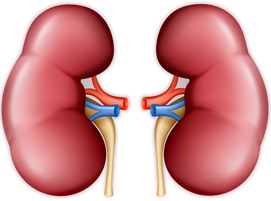
\includegraphics[width=0.15\textwidth]{kidney.png}
    \caption{Kidneys}
\end{wrapfigure}
The kidneys are a pair of organs, with the shape of a bean, located on either side of the spine, below the ribs and behind the belly. Among their functions, filtering the blood is one of them: the kidneys filter over 180 liters per day producing an ultrafiltrate that goes through other processes such as reabsorption, secretion and excretion. In the end, this leads to the production of urine. The "chronic kidney disease" is the malfunction of the kidneys in carrying out their basic tasks; this can be caused by many different conditions such as type 1 or type 2 diabetes, high blood pressure, vesicoureteral or frequent kidney infections.

\subsection{Glomerular Filtration Rate}
The Glomerular Filtration Rate is a value that represents the stage of the disease; it can be calculated in many ways, for example by evaluating the amount of creatinine that is removed from the blood. If a patient removes 1440 mg in 24 h, this is equivalent to removing 1 mg/min. If the blood concentration is 0.01 mg/mL (1 mg/dL), then one can say that 100 mL/min of blood is being "cleared" of creatinine, since, to get 1 mg of creatinine, 100 mL of blood containing 0.01 mg/mL would need to be cleared.
\begin{table}[htb]
\centering
\begin{tabular}{|ccc|}
\hline
\textbf{Stage} & \textbf{Description} & {$\mathbf {GFR \left( m L/min\textbf{ per } 1.73m^{2} \right)}$} \\ \hline
1 & Kidney damage with normal or increased GFR & $\geq 90$ \\ \hline
2 & Kidney damage with mildly decreased GFR & 60 - 89 \\ \hline
3 & Moderately decreased GFR & 30 - 59 \\ \hline
4 & Severely decreased GFR & 15 - 29 \\ \hline
5 & Kidney failure & \textless 15 (or undergoing dialysis) \\ \hline
\end{tabular}
\caption{Evaluation of Chronic Renal Disease}
\label{my-label}
\end{table}




\subsection{Our purpose}
\textit{The healthcare industry collects huge amounts of healthcare data which, unfortunately, are not “mined” to discover hidden information for effective decision making. The discovery of hidden patterns and relationships often goes unexploited. Advanced data mining techniques can help remedy this situation} \cite{SITE} and contributes to effective prediction, exploration, diagnosis and decision making. Machine learning techniques can provide tools to handle these processes. We aim to find out if patients, according to their medical values, have developed Chronic Kidney Disease or not, even in case the Data-Set is not totally complete. 
In order to perform analysis, prediction, diagnosis and decision making requires we need as much data as possible. Such data allow to perform \textbf{CART} algorithms (Classification And Regression Tree), available in the Python Scikit Learn library, more precisely. If some data are missing, we can obtain them with regression algorithms.

\pagebreak

\section{Regression on data}
\subsection{Cleaning and managing the data}
 It is crucial to have a Data-Set without typing or conversion errors: for this reason, the first task is to detect and delete all those elements that alter the file's structure. The second task is to fill all the "empty features" with the \textbf{NaN} (not a number).
To perform the regression, we will use a Data-Set provided by the University of California \cite{DS}. We will only consider patient records containing at least 20 features. Since many features are nominal (such as the ones in the \textbf{Table} \textbf{\ref{table1}}) we opted for a numerical notation as follows:

\begin{table}[h]
\resizebox{\textwidth}{!}{%
\begin{tabular}{|c|c|c|c|c|c|c|c|c|c|c|}
\hline
\textbf{Nominal description} & normal & abnormal & present & not present & yes & no & poor & good & CKD & NOT CKD \\ \cline{1-1}
\textbf{Numerical conversion} & 0 & 1 & 1 & 0 & 1 & 0 & 0 & 1 & 1 & 0 \\ \hline
\end{tabular}%
}
\caption{Conversion of the descriptions in binary values}
\label{table1}
\end{table}

\subsection{The Algorithm}
We modeled our Data-Set as a matrix of \textbf{400} rows (number of patients) and \textbf{25} columns (features of the patients). The data matrix \textbf{X} contains only patients records with 25 registered features and with normalized values. The data train matrix is the full Data-Set \textbf{X} without the column of the first occurrence of a \textbf{NaN}, which is the column $\mathbf{y_{train}}$.
We found the optimum weight vector \textbf{w} of linear regression by using Ridge Regression with a fixed \textbf{Lagrangian multiplier} $\mathbf{\lambda = 10}$. Finally, we regressed the missing value (denormalized) in the row where it was initially missing. This method is then reiterated to regress more missing features.




\section{Results}
\subsection{Discussion on the results of the "Decision Tree"}

The divisive hierarchical algorithm used generates alternatively 3 different binary trees, as it is shown in \textbf{Figure \ref{fig:trees}}. "\textit{Hemoglobin}" is the feature that has a bigger importance in defying the state of the patient; its threshold is, in all the decision trees, \textbf{12.95 g/dL}, a reasonable value considering the expected one for a healthy adult (12 - 16 g/dL). In all the decisive trees created "\textit{Specific Gravity}" and "\textit{Albumin}" are respectively second and third in importance to determinate the presence or not of the disease. The less important feature in each tree changes: in the first one it is "\textit{White Blood Cell Count}", in the second it is "\textit{Pedal Edema}" while in the third it is "\textit{Serum Creatinine}".
\begin{table}{}
\centering
\begin{tabular}{cccc}
\hline
\textbf{Feature} & \textbf{Tree 1} & \textbf{Tree 2} & \textbf{Tree 3} \\ \hline
\multicolumn{1}{|c|}{Hemoglobin} & \multicolumn{1}{c|}{67,39\%} & \multicolumn{1}{c|}{67,39\%} & \multicolumn{1}{c|}{67,39\%} \\ \hline
\multicolumn{1}{|c|}{Specific Gravity} & \multicolumn{1}{c|}{24,59\%} & \multicolumn{1}{c|}{24,59\%} & \multicolumn{1}{c|}{24,59\%} \\ \hline
\multicolumn{1}{|c|}{Albumin} & \multicolumn{1}{c|}{5,41\%} & \multicolumn{1}{c|}{5,41\%} & \multicolumn{1}{c|}{5,41\%} \\ \hline
\multicolumn{1}{|c|}{White Blood Cell Count} & \multicolumn{1}{c|}{2,59\%} & \multicolumn{1}{c|}{0} & \multicolumn{1}{c|}{0} \\ \hline
\multicolumn{1}{|c|}{Pedal Edema} & \multicolumn{1}{c|}{0} & \multicolumn{1}{c|}{2,59\%} & \multicolumn{1}{c|}{0} \\ \hline
\multicolumn{1}{|c|}{Serum Creatinine} & \multicolumn{1}{c|}{0} & \multicolumn{1}{c|}{0} & \multicolumn{1}{c|}{2,59\%} \\ \hline


\end{tabular}
\caption{Feature's importance}
\label{table2}
\end{table} 


\begin{figure}[H]
\centering
\begin{center}
\subfloat[][\emph{Tree 1}\label{fig:a}]
{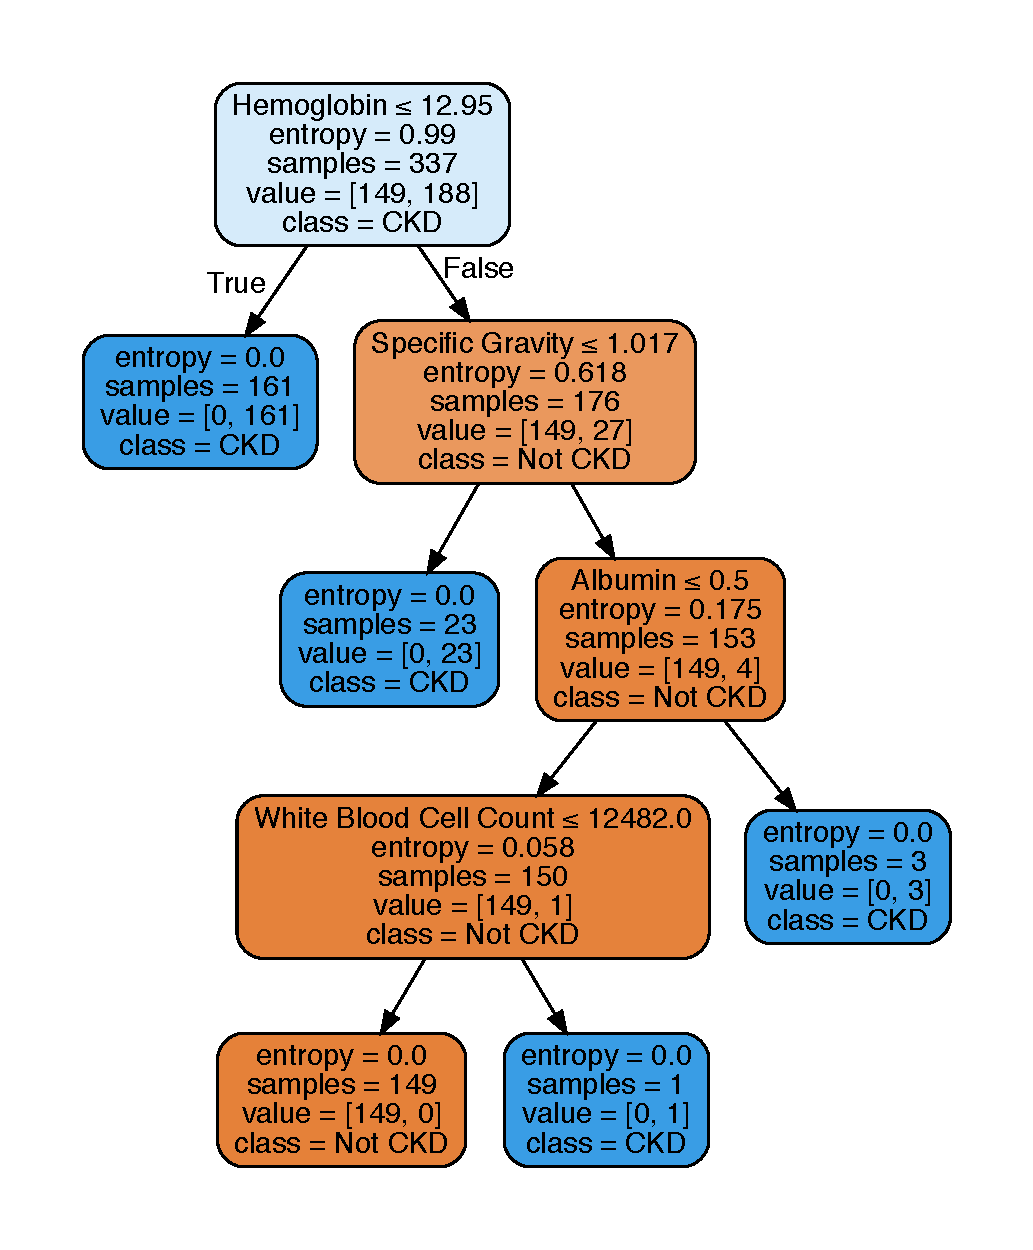
\includegraphics[width=.34\textwidth]{0Tree.pdf}}
\subfloat[][\emph{Tree 2}\label{fig:b}]
{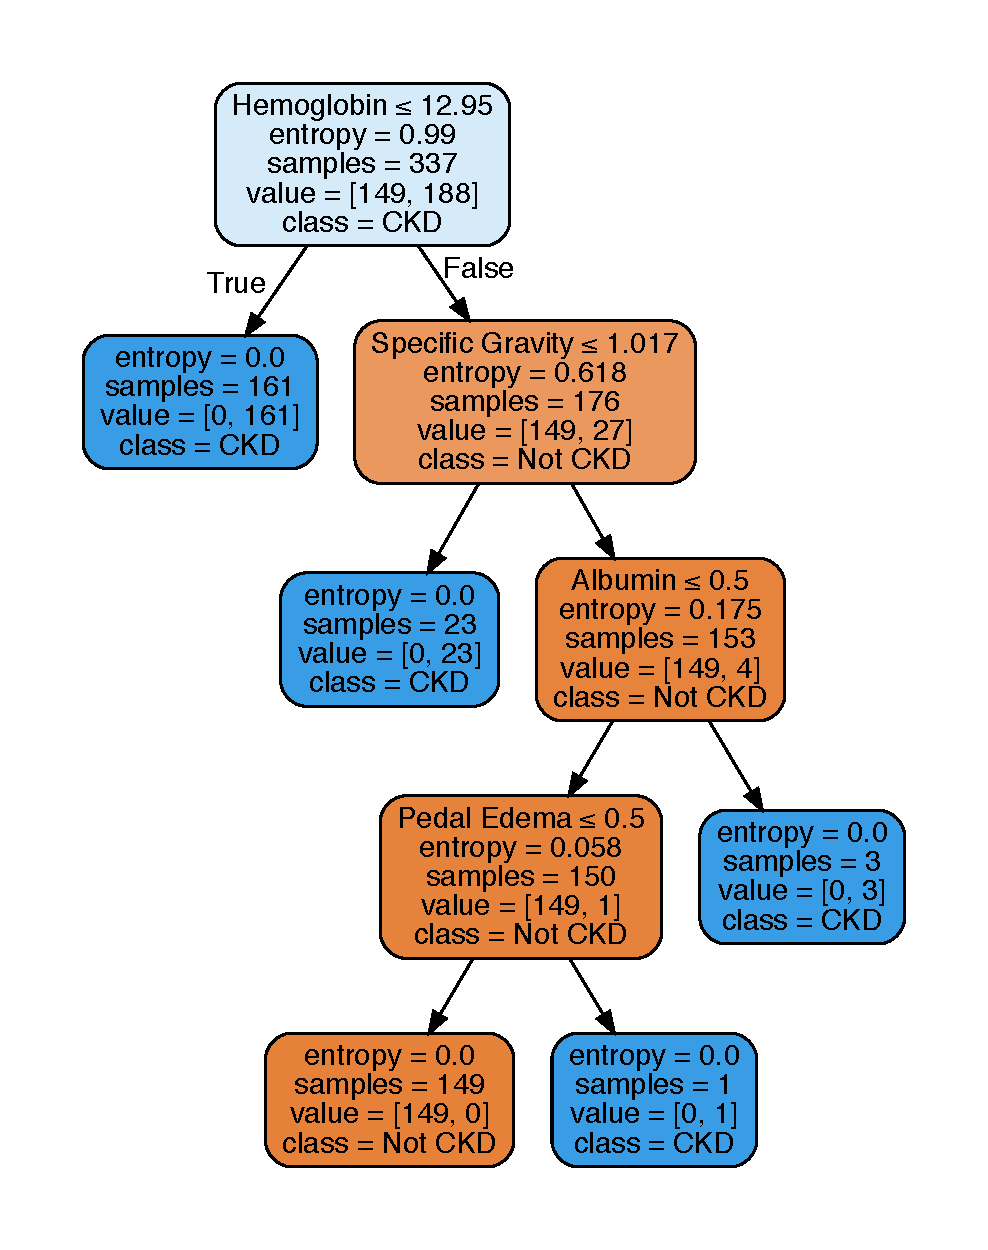
\includegraphics[width=.34\textwidth]{1Tree.pdf}}
\subfloat[][\emph{Tree 3}\label{fig:c}]
{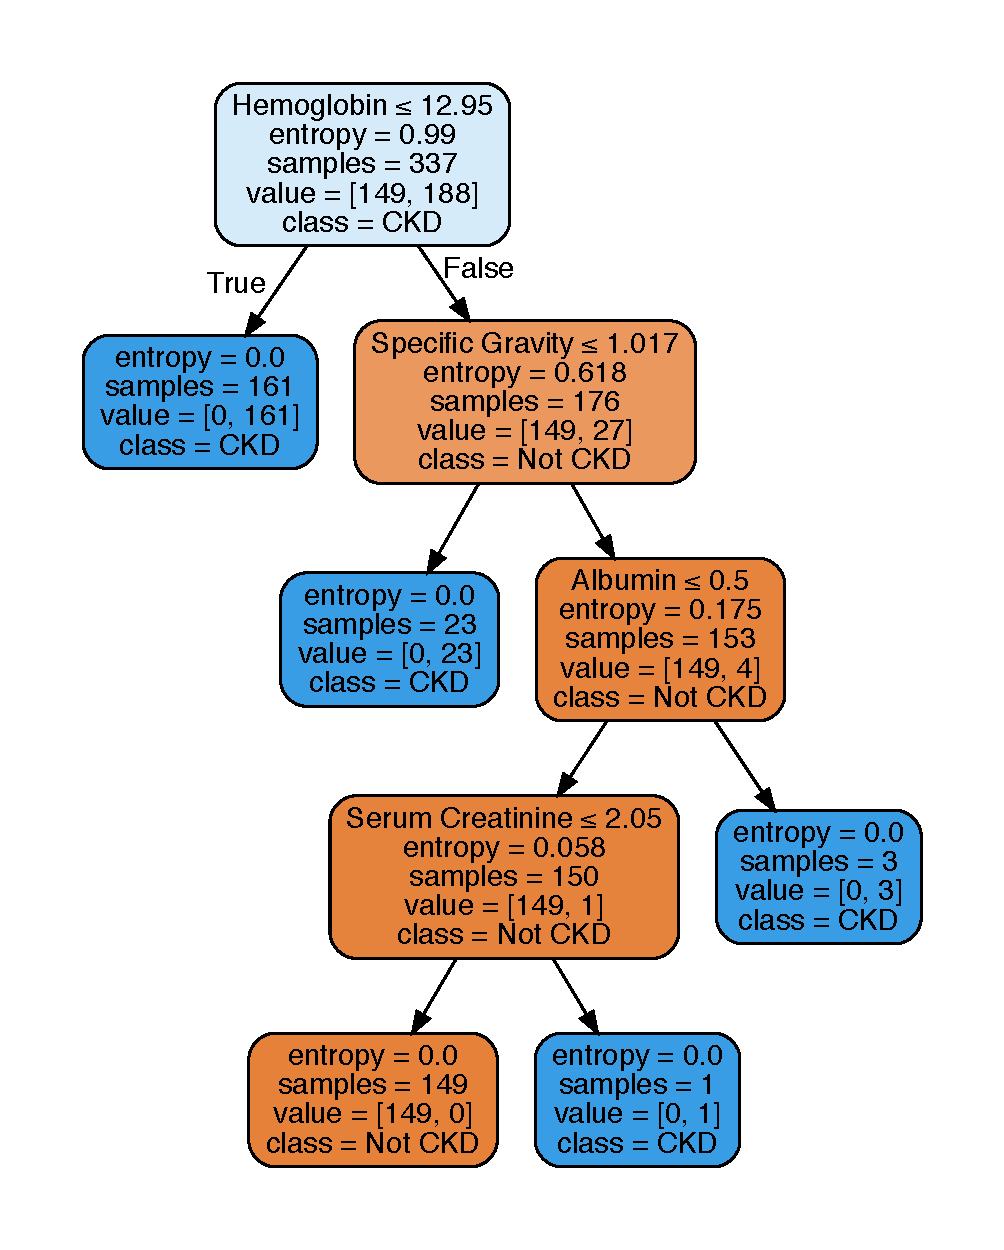
\includegraphics[width=.34\textwidth]{2Tree.pdf}}
\caption{Decision Trees for different random states}
\label{fig:trees}
\end{center}
\end{figure}

\subsection{Conclusions}
Available data are not sufficient for a precise account of a patient's health state since hemoglobin is considered as the most important element for the diagnosis of kidney failure. 
According to specialists, the value of albumin is the most important feature to be taken into consideration in the data set. The filtration of liquids that takes place in the kidney glomerulous allows smaller molecules to pass. Proteins, such as albumin, do not pass as they are normally bigger. If the opposite happens, kidneys are not working properly. In the second phase of filtration, filtered liquids except albumin are reabsorbed into the tubule. This causes a lack of albumin in the body. Albumin is necessary for oncotic pressure, which allows the re-absorption of liquids at the level of capillary venules. If this physiological process is altered, the level of liquids within tissues increases. Physicians can find evidence of alteration in case of a pedal edema. 
Another signal of kidney failure is an increase of serum creatinine over a certain threshold. However, this has to be put in context because excess of serum creatinine can be caused by physical over-training as well.
Finally, it may be concluded that the algorithm does not work properly if data availability is poor. For this reason, the glomerular filtration rate is still the most reliable signal of kidney failure.

\begin{thebibliography}{99}
\bibitem{SITE} \texttt{Prediction System Using Data Mining Techniques}\\\url{http://paper.ijcsns.org/07_book/200808/20080849.pdf}
\bibitem{DS} \texttt{Chronic Kidney Disease Data Set - UCI}\\\url{https://archive.ics.uci.edu/ml/datasets/chronic_kidney_disease}
\end{thebibliography}


\pagebreak

\end{document}
